%\begin{savequote}[6cm]
%<< Some other great quote  >>
%\qauthor{Someone}
%\end{savequote}
\chapter{État de l'art}\label{chap:rw}
\chaptertoc


\begin{figure}[ht]
  \centering
  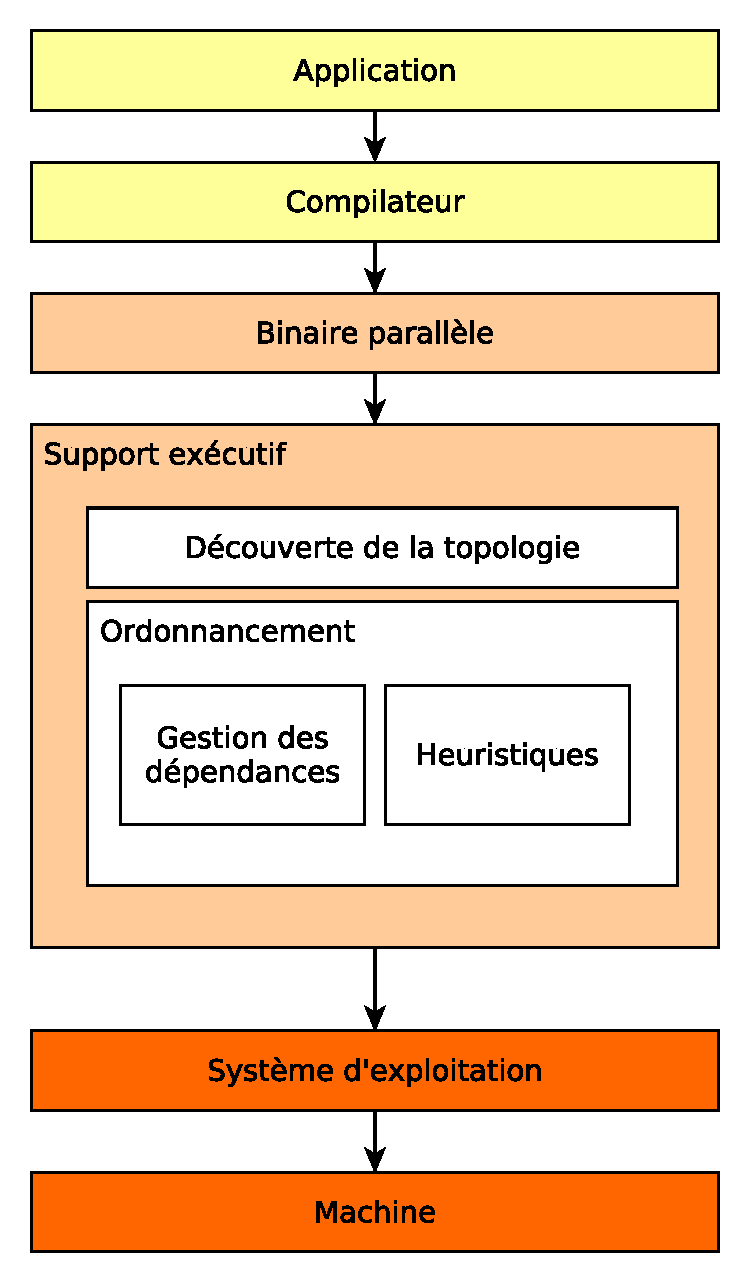
\includegraphics[width=0.5\textwidth]{schema-application-os}
  \caption{Schéma des acteurs impliqués dans l'exécution d'une application}\label{fig:rw:application-os}
\end{figure}

L'objectif de ce chapitre est de donner un aperçu des travaux existants dans le contexte de cette thèse.
Comme on peut le voir sur la figure~\ref{fig:rw:application-os}, un certain nombres d'acteurs sont impliqués dans l'exécution d'une application.

Les parties application, système d'exploitation, et matériel ont été traitées dans le chapitre précédent~; ce chapitre ce concentrera dans un premier temps sur une partie précise des supports exécutifs, en abordant les différentes techniques d'ordonnancement présentes dans l'état de l'art pour cibler spécifiquement les machines NUMA, puis nous regarderons en détails certains supports exécutifs existant, et enfin nous ferons un point sur les compilateurs OpenMP.






\section{Architectures à mémoire partagée}\label{sec:context:numa}


Les architectures à mémoire partagée ont subit des changements majeurs liés à l'évolution des processeurs.
L'augmentation du nombre de cœurs par processeur a introduit des problèmes d'accès à la mémoire centrale : dans une architecture composée d'une unique mémoire, plusieurs cœurs cherchant à accéder à la mémoire vont rentrer en concurrence et introduire de la contention et donc des délais dans l'accès à la mémoire, ce qui pénalise formtement les performances.

Pour pallier ce problème, les constructeurs ont divisé la mémoire centrale en plusieurs parties physiquement distinctes, appelées \emph{nœuds}.
Le nœud NUMA est le composant de base pour une architecture NUMA.
Chaque nœud est constitué d'une partie de la mémoire centrale, d'un contrôleur local d'accès à ce bloc mémoire, ainsi que d'un certain nombre de cœurs de calcul.
L'ensemble des nœuds de la machine sont ensuite reliés entre eux par un réseau d'interconnexion.
La topologie de l'interconnexion ne permet généralement pas d'avoir des nœuds équidistants, ce qui introduit une hiérarchie mémoire.

Malgré le fait que les différentes parties de l'architecture soient physiquement séparées, le système d'exploitation voit l'ensemble comme une unique machine.

Nous décrivons dans un premier temps les caractéristiques techniques communes d'un processeur multicœur d'un nœud dans les sections~\ref{sec:context:numa:cache}, et~\ref{sec:context:numa:node}, puis celles des systèmes d'interconnexion des nœuds dans la section~\ref{sec:context:numa:interconnect}.
Elles ont une influence directe sur le comportement du nœud au sein de la machine.

\subsection{Caches des processeurs}\label{sec:context:numa:cache}

Le cache est une mémoire pour laquelle le temps d'accès est bien meilleur que pour la mémoire centrale, mais dont la capacité est beaucoup plus restreinte. Il peut être spécifique à un cœur du processeur, ou partagé par plusieurs d'entre eux.

\subsubsection{Fonctionnement}

Au niveau des accès le fonctionnement d'un cache est légèrement différent de celui de la mémoire centrale : plutôt que de lire uniquement un octet, c'est généralement une partie fixe de la mémoire contenant cet octet qui est chargée.
On appelle cette quantité une \emph{ligne de cache}, et un exemple de taille standard pour une ligne de cache est 64 octets (8 nombres réels double précision).

Lorsqu'une instruction demande le chargement d'une valeur située en mémoire, le contrôleur du cache reçoit la requête du processeur, détermine la ligne de cache correspondante à partir de l'adresse demandée, et effectue l'une des deux opérations suivantes :
\begin{description}
  \item [Cache hit :] si la ligne correspondante est déjà présente dans le cache la donnée est directement retournée au cœur.
  \item [Cache miss :] si la ligne n'est pas présente le contrôleur de cache va charger la valeur depuis la mémoire centrale vers le cache, et retourner la valeur au cœur.
\end{description}

%(je vire ça vu qu'on ne parle de niveaux de cache que plus tard) Si le cœur a accès à plusieurs niveaux de cache, la requête est transférée au niveau supérieur, et seul le dernier niveau effectue la requête à la mémoire centrale.
Une fois qu'une ligne est chargée dans le cache, elle n'y reste pas de manière permanente, plusieurs raisons décrites ci-après peuvent entraîner son \emph{éviction} du cache :

\begin{itemize}
  \item Le maintien de la cohérence : lorsqu'un cœur modifie une ligne de cache dans son propre cache, cette même ligne est \emph{invalidée} dans les caches des autres processeurs qui en disposent d'une version.
Si un processeur essaie de faire un accès sur une ligne invalidée, elle sera rechargée depuis la mémoire centrale, générant un \emph{cache miss}.
  \item Le dépassement de la capacité du cache : il est assez commun que l'ensemble des données manipulées par le programme ne tienne pas dans le cache.
Lorsqu'une requête est effectuée sur une ligne, qu'elle n'est pas présente dans le cache, et que le cache est plein, le contrôleur choisira une ligne à évincer du cache pour faire de la place à la nouvelle ligne.
Le choix de la ligne à évincer est un sujet très étudié, et le prochain paragraphe revient sur les politiques d'éviction communément utilisées.
  \item Le conflit d'adresse : dans certains modèle de caches, certaines lignes correspondant à des adresses mémoires doivent être stockées dans le même emplacement du cache.
    Si elles sont requises alternativement pendant l'exécution du programme, elles se sortiront mutuellement du cache.
    Ce problème dépend directement de l'\emph{associativité} du cache, qui est traitée dans le paragraphe suivant.
\end{itemize}



\subsubsection{Associativité}

Le cache ne pouvant être suffisamment grand pour contenir toute la mémoire, il faut pouvoir déterminer l'association entre l'adresse d'une ligne dans la mémoire centrale et son emplacement dans le cache.
Il y a trois grandes catégories d'associativité utilisées par les caches :
\begin{itemize}
  \item Les caches à association directe (\emph{direct-mapped cache}) : dans ce système, chaque ligne de la mémoire est associée à exactement un emplacement dans le cache.
    Ce système est simple, propose le meilleur temps de réponse, mais est peu prévisible et à taille identique est moins efficace que les deux autres catégories.
  \item Les caches complètement associatifs (\emph{fully associative cache}) : dans ce système, chaque ligne de la mémoire peut être associée à n'importe quel emplacement dans le cache.
    Cela permet de maximiser l'utilisation de l'espace disponible, mais cela induit un coût supplémentaire pour déterminer l'association entre une ligne et son emplacement.
  \item Les caches N-associatifs (\emph{N-way associative cache}) : ce système est un compromis entre les deux précédents.
    Chaque ligne de la mémoire peut être associée à exactement N emplacements dans le cache.
    Cela implique un certain nombre d'opérations sur les adresses des lignes, et l'espace pris par le composant ainsi que le temps d'accès moyen dépend directement de la valeur de N.
\end{itemize}

Hill et al.~\cite{Hill1989} (Table III) illustre l'impact de l'associativité sur la proportion de cache miss et catégorise son origine (conflit d'adresse, défaut de capacité du cache, chargement normal de la donnée).
Cela permet de dégager deux observations : d'une part qu'augmenter l'associativité permet de diminuer les cache miss.
D'autre part que les défauts de cache ayant une forte associativité sont quasi exclusivement dus à la capacité du cache, alors que pour les caches à association directe les conflits d'adresse sont une part non négligeable des cache miss.

\subsubsection{Niveaux de caches}

Il y a en général 3 niveaux de cache dans ces architectures :
\begin{itemize}
  \item L1 : C'est le cache le plus "proche" du CPU, mais aussi le plus petit - typiquement quelques Ko. Il est généralement découpé en deux parties distinctes : une partie pour les instructions, une autre pour les données.
  \item L2 : Ce cache est physiquement plus éloigné du processeur et présente une latence d'accès plus importante que le L1, mais propose une plus grande capacité de mémoire. Il a un ordre de grandeur de quelques centaines de Ko.
  \item L3 : Ce cache est généralement le cache de dernier niveau - \emph{Last Layer Cache (LLC)} - sur un processeur. La latence pour y accéder est plus importante que le L2, mais sa capacité est bien supérieure, pouvant en général atteindre plusieurs Mo.
\end{itemize}

En fonction des fabricants, ces caches peuvent être soit \emph{inclusifs} (c'est-à-dire que toutes les données présentes dans le L1 sont également présentes dans le L2), ou \emph{exclusifs} (c'est-à-dire qu'une donnée est garantie de n'être présente que dans l'un des caches).

Au sein d'un nœud, le L3 est généralement partagé par tous les cœurs, alors que les caches L1 et L2 sont spécifiques à un cœur.

\begin{figure}[ht]
  \centering
  \includegraphics{processor_small}
  \caption{Schéma d'un processeur multicœurs}\label{fig:context:schema-caches}
\end{figure}

La figure~\ref{fig:context:schema-caches} décrit la hiérarchie typique d'un processeur multicœurs que l'on peut trouver sur un nœud NUMA.
Dans cet exemple, le processeur dispose de 8 cœurs, et chaque cœur dispose d'une cache L1 indépendant pour les données et les instructions (32 Ko chacun), d'un cache L2 (256 Ko), et d'un cache L3 partagé avec 7 autres cœurs (20 Mo).


En général les développeurs d'applications pour le HPC accordent beaucoup d'attention à l'optimisation de leur application, pour que les parties de code séquentiel critiques utilisent des données qui puissent être contenues dans le L1/L2.
De même, beaucoup d'optimisations au sein des compilateurs visent également cet objectif.

Lorsqu'il s'agit de cibler des architectures NUMA, on va tout particulièrement s'intéresser au L3, qui représente la mémoire la plus rapide accessible par tous les cœurs d'un même nœud.

\begin{todo}
TODO : ref + paragraph sur les caches configurables du ryzen.
Pas trouvé de ref sur le ryzen parlant de cache configurable, mais j'ai trouvé Jenga : http://people.csail.mit.edu/sanchez/papers/2017.jenga.isca.pdf
\end{todo}

\begin{table}[ht]
\def\arraystretch{1.5}
\centering
\begin{tabular}{|c||c|c|c|c|}\hline
  Cache & \multicolumn{2}{c|}{Intel Sandy Bridge} & \multicolumn{2}{c|}{Intel Broadwell}  \\ \cline{2-5} 
 & Latence & Bande passante & Latence & Bande passante \\ \hline
 L1 & 1.6 ns & 16 Go/s & 1.8 ns & 32 Go/s \\ \hline
 L2 & 5.0 ns & 14 Go/s & 5.4 ns & 17 Go/s \\ \hline
 L3 & ~20 ns & 8 Go/s & ~24 ns & 9 Go/s \\ \hline
 RAM & ~90 ns & 4 Go/s & ~140 ns & 7 Go/s \\ \hline
\end{tabular}
\caption{Tableau synthétiques des latences et bande passante en fonction du niveau de cache et du processeur}\label{tab:synthese-processeurs}
\end{table}

Afin de donner un ordre d'idée des latences et bande passantes sur les différents processeurs, le tableau~\ref{tab:synthese-processeurs} récapitule les chiffres en fonction de la génération du processeurs.
Les mesures ont été faites à l'aide de l'outil LMbench~\cite{McVoy1996}. Pour la latence, les temps considérés sont ceux du benchmark |lat_mem_rd| avec un accès aléatoire à la mémoire.
Pour la bande passante les temps considérés sont ceux du benchmark |bw_mem|, en utilisant un équivalent de |memcpy|.
Pour la latence, tout effet potentiel du prefetcher est annulé par l'utilisation de \emph{pointer chasing} (l'adresse de la case suivante à charger est située dans la case courante), ce qui n'est pas le cas pour la bande passante.

Comme on peut le voir sur ces chiffres, le coût d'accès à la mémoire principale est prohibitif par comparaison aux différents caches, y compris le L3.
Les différentes caractéristiques de ces processeurs et des machines sur lesquels ils sont intégrés seront étudiées en détails dans la section~\ref{sec:contribs:machines}.

\subsubsection{Politiques d'éviction}

Le choix de la ligne de cache à remplacer lorsque le cache est plein a un impact direct sur les performances, et les politiques de remplacement ont été très étudiées par les différents acteurs de la communauté académique et industrielle.

La politique optimale serait de remplacer la ligne qui sera réutilisée le plus tard, mais ce genre de clairvoyance est impossible à implémenter en pratique.
Un certain nombre d'alternatives ont donc été imaginées, et sont décrites ci-après :
\begin{itemize}
  \item Random : cette politique choisi une ligne à remplacer au hasard. Sa simplicité la rend simple à implémenter en pratique, et a notamment été utilisée dans les processeurs ARM Cortex-R~\cite{ARM-Cortex-R}.
  \item First-In First-Out : comme son nom l'indique, la ligne remplacée est la première qui est rentrée dans le cache parmi celles présentes.
  \item Least Recently Used (LRU) : dans cette politique, chaque ligne dispose de plusieurs bits représentant la date de la dernière utilisation de cette ligne. La ligne remplacée est celle ayant été utilisée il y a le plus longtemps.
  \item Pseudo-LRU : cette politique offre une version dégradée permettant de gérer des caches de grandes tailles.
Lorsque l'associativité du cache dépasse un certain seuil, le coût d'implémentation de LRU devient trop important~\cite{Kedzierski2010}, l'alternative proposée par les politiques pseudo-LRU est donc de remplacer une ligne parmi celles utilisées il y a le plus longtemps.
Cela permet de limiter le nombre de bits nécessaire pour tracer les lignes à remplacer potentielles.
  \item Autres politiques adaptatives : dans le cas spécifique du cache de dernier niveau (LLC), certains fabriquants comme Intel utilisent des politiques adaptatives présentées comme supérieures à Pseudo-LRU, prenant en compte la fréquence à laquelle sont utilisées certaines lignes de caches.
    \emph{Dynamic Re-Referency Interval Prediction} en est un exemple, qui a été présenté parmi d'autres par Jaleel et al.~\cite{Jaleel2010}.
\end{itemize}

La politique pseudo-LRU semble être la plus utilisée par les fabricants de processeurs tous niveaux de cache confondus. Al-Zoubi et al.~\cite{Al-Zoubi2004} proposent une évaluation complète et détaillée de l'impact des politiques d'éviction en fonction de l'associativité du cache, justifiant le choix des constructeurs.



\subsection{Autres caractéristiques matérielles des processeurs}\label{sec:context:numa:node}

En plus des caches qui nous intéresseront tout particulièrement dans la suite de ce manuscrit, les processeurs ont également d'autres composants matériels dont il est important d'avoir conscience, mais qui ont une place plus limitée dans le contexte de cette thèse : il s'agit des instructions vectorielles et de l'hyperthreading, décrit ci-après.

\subsubsection{Instructions vectorielles}\label{sec:context:numa:simd}

Le concept de vectorisation est l'action d'appliquer une même instruction sur plusieurs données (ou un \emph{vecteur} de données) nécessitant la même opération.
Ce type d'instructions est appelée SIMD, pour \emph{Single Instruction Multiple Data}.

Afin d'illustrer ce point, il suffit d'imaginer que l'on souhaite additionner deux vecteurs d'entiers :
\begin{lstlisting}
int vecteur_a[8] = { 1 };
int vecteur_b[8] = { 1 };
int addition[8];
for (int i = 0; i < 8; i++) {
  addition[i] = vecteur_a[i] + vecteur_b[i];
}
\end{lstlisting}

Exécuter la boucle complète effectuerait 8 additions sur des entiers.
En supposant que la largeur des registres (et des instructions) du processeur est de 64 bits, et que la taille d'un |int| est 32 bits, on "gaspillerait" en fait 32 bits par addition.

Étant donné que l'on souhaite effectuer la même opération (une addition), sur des éléments indépendants du tableau, on peut alors aisément grouper deux additions successives dans la même instruction : il suffit de mettre un entier de 32 bits sur la partie haute du registre, et un deuxième entier sur la partie basse, d'effectuer l'instruction, et de faire l'opération inverse pour stocker le résultat dans le tableau.
De plus la vectorisation permet au processeur d'optimiser la décomposition de l'instruction en micro opérations et donc l'utilisation du pipeline.
Au final on divise le nombre d'itérations, mais aussi le nombre d'accès mémoire et d'opérations par 2.


\begin{todo}
  j'ai pas trouvé la ref des procs vectoriels sur ACM, (re)demander à Thierry
\end{todo}

Des extensions au jeu d'instructions x86 ont été créées afin de pouvoir opérer sur des éléments plus larges que 64 bits, et la plupart des architectures des processeurs récents utilisent des registres plus larges que le type le plus large en C (|long long|, 64 bits).
La première d'entre elles, SSE (\emph{Streaming SIMD Extensions}), a été introduite par Intel dès 1999 et a évolué régulièrement, agrandissant progressivement la taille des registres jusqu'à l'extension AVX-512, permettant d'effectuer des instructions sur des registres de 512 bits.

La plupart des processeurs actuels (depuis les Sandy Bridge d'Intel, et les Bulldozer d'AMD, en 2011) supportent au moins l'extension AVX avec des registres de 128 bits.

\subsubsection{Hyperthreading}

Chaque cœur possède un certain nombre d'UAL (Unité Arithmétique et Logique) qui lui sont privées. Lorsqu'il est en attente d'une donnée de la mémoire centrale, ces UALs ne sont pas utilisées, et des cycles CPU sont donc "perdus" à ne rien faire.

Afin de maximiser l'utilisation de ces ressources, certains processeurs Intel sont équipés de la technologie \emph{hyperthreading}.
Le concept est assez simple : avoir deux cœurs logiques (\emph{hyperthreads}) associés à un seul cœur physique.
De cette manière lorsqu'un thread est en attente sur une donnée (par exemple lors d'un chargement d'une donnée depuis la mémoire), le second peut profiter des UALs disponibles.

Pour des tâches peu gourmandes en ressources ou utilisant beaucoup de données, cela peut effectivement se traduire par un gain de performances, mais pour le cas des applications HPC il faut regarder le type d'applications utilisées pour savoir si on peut espérer un gain ou non.
En particulier les caches L1 et L2 sont partagés par les deux hyperthreads, donc si le code séquentiel généré est optimisé pour les tailles de caches correspondant, exécuter le même type de code séquentiel sur deux hyperthreads peut entrainer du \emph{cache trashing}.
Au meilleur des cas l'hyperthreading améliorera les performances mais ne sera pas forcément très efficace, atteignant par exemple entre 2.3 et 3.3 de speed-up pour 4 hyperthreads par cœur~\cite{Jeffers2016} sur les derniers processeurs d'Intel, les Xeon Phi.
Si l'application est très intensive en calcul et utilise au maximum les UALs, l'hyperthreading n'apportera pas grand chose, voire rien.

L'hyperthreading est généralement une option que l'on peut désactiver dans le BIOS de la machine, ou éviter en plaçant correctement les threads de son application.


\subsection{Interconnexion des nœuds}\label{sec:context:numa:interconnect}

L'une des parties majeures d'une machine NUMA est le système d'interconnexion entre les différents nœuds.
C'est cette partie qui va déterminer à quel point cela va être couteux d'accéder à la mémoire située sur un nœud distant, et donc à quel point l'aspect NUMA de la machine va impacter les performances d'une application.
Dans la majorité des cas, ce système d'interconnexion est \emph{cache-coherent}, c'est à dire que la cohérence de cache est assurée entre les différents nœuds par le matériel, et n'est pas la responsabilité du programmeur ou du support exécutif.
L'impact sur les performances peut être lié à la fois au protocole de cohérence de caches utilisé, ainsi qu'à la topologie de l'interconnexion des nœuds.


\subsubsection{Protocoles de cohérence de cache}

Le nombre de caches utilisés dans une machine NUMA peut être important, et la même ligne de la mémoire peut être présente dans plusieurs caches en même temps.
Il est important que l'état des différentes copies soit cohérent : par exemple si une ligne a été écrite et modifiée, les copies de cette ligne dans les autres caches doivent être mises à jour.

La plupart des protocoles se basent sur un ensemble d'états possibles pour une ligne de cache :

\begin{description}
  \item [Modified (M) :] la ligne a été modifiée dans le cache. Les données dans cette ligne ne sont donc pas cohérentes avec la mémoire principale. Quand la ligne est évincée, elle doit être écrite dans la mémoire principale.
  \item [Shared (S) :] la ligne est <<propre>> (non modifiée), elle existe dans d'autres caches mais est en lecture seule dans le cache courant. Cette ligne peut être évincée sans autre action.
  \item [Invalid (I) :] la ligne est soit absente du cache courant ou a été invalidé par un autre cache. Elle doit être récupérée depuis la mémoire principale (ou un autre cache qui en possède une copie valide).
\end{description}

Cet ensemble d'états de base forme le protocole \emph{MSI}, qui a ensuite été étendu avec plusieurs autres états :

\begin{description}
  \item [Exclusive (E) :] la ligne est présente uniquement dans le cache courant et elle est <<propre>>.
  \item [Owned (O) :] la ligne est présente dans plusieurs caches dans un état valide, mais seul le cache courant peut y effectuer des modifications.
    Cet état permet de partager des lignes qui ont été modifiées sans passer par une ré-écriture dans la mémoire centrale : le cache qui possède la ligne est responsable de fournir une version à jour, et d'écrire la ligne dans la mémoire centrale lorsque que la ligne est évincée.
  \item [Forward (F) :] cet état est similaire à l'état \emph{Shared}, mais indique au cache courant qu'il est responsable de satisfaire une requête en lecture sur la ligne.
\end{description}

Intel Quick Path Interconnect~\cite{Ziakas2010} (QPI) est le système d'interconnexion utilisé dans les machines d'expérimentation que nous avons utilisé, et qui sont décrites dans la section~\ref{sec:contribs:machines}.
Il implémente le protocole MESIF. Du à l'introduction de l'état \emph{F}, ce protocole est avantageux lorsque la latence de cache à cache est bien plus faible que la latence d'accès à la mémoire principale.

Pour implémenter ce protocole, il existe deux types de mécanismes :

\begin{itemize}
  \item À base de Snooping : chaque cache observe le trafic sur le bus mémoire pour des requêtes qui concerneraient les lignes de caches dont ils possèdent une copie. Un composant dédié peut effectuer un premier filtre pour restreindre le trafic lié au mécanisme de snooping. Néanmoins ce type de mécanismes ne passent pas bien à l'échelle, et aurait du mal à obtenir de bonne performance dans les architectures NUMA, où le nombre de caches est important.

  \item À base de répertoires : la donnée est placée dans un répertoire qui maintien la cohérence entre les caches. Chaque cache ne peut pas accéder directement à la mémoire principale mais doit passer par le répertoire.
\end{itemize}

Le QPI utilise un mix des deux mécanismes : il utilise des \emph{home agents} - comparables à des répertoires - qui sont les principales autorités pour fournir une version du cache depuis la mémoire principale.
Il utilise ensuite du \emph{snooping} pour satisfaire les requêtes des différents \emph{caching agents} (les entités qui possèdent un cache, telles que les processeurs).

Le QPI peut fonctionner avec deux modes de \emph{snooping} :
\begin{description}
  \item [Source snooping :] le \emph{caching agent} envoie la requête à tout le système. Les autres \emph{caching agent} peuvent répondre à la requête s'ils possèdent une version de la ligne de cache dans un état compatible. Le \emph{home agent} responsable de la ligne mémoire doit fournir une copie propre de la ligne de cache si besoin, et résoudre les conflits s'ils apparaissent.
  \item [Home snooping :] le \emph{caching agent} envoie la requête au \emph{home agent}, qui envoie ensuite une requête aux \emph{caching agents} qui possèdent une copie de la ligne et peut commencer à charger la ligne depuis la mémoire. L'un des \emph{caching agents} possédant la ligne et/ou le \emph{home agent} peut ensuite envoyer la réponse.
\end{description}

Le mode \emph{source snooping} a une latence plus faible que le mode \emph{home snooping}, mais passe moins bien à l'échelle.
C'est donc ce dernier qui est le plus adapté à un environnement NUMA, puisqu'il limite le nombre de requêtes envoyés sur le bus mémoire, et économise donc de la bande passante.


\subsubsection{Topologies}
\begin{todo}
  décrire le facteur NUMA et inclure des chiffre (reprendre graphe 2.1.2 plus bas)
\end{todo}

La topologie du système d'interconnexion peut être très différente d'une machine à une autre, et de multiples exemples existent dans les machines commercialisées.
Il existe des topologies plates, où chaque nœud est directement connecté aux autres (TODO: ref graph 2.1.2), des topologies où des couples de nœuds sont groupés entre eux et peuvent passer par un ou deux niveaux d'interconnexion (TODO: ref graph idchire).

Le nombre de rebonds - \emph{hops} - à effectuer avant d'accéder à la mémoire demandée impacte directement la latence et la bande passante, comme le montre le tableau comparatif de la figure~(TODO).

Chiffres :
même noeud: 2.11 GB/s
noeud meme group: 1.50 GB/s
groupe proche: 1.28 GB/s
groupe loin: 1.06 GB/s

GRAPHE : 2.1.2 les chiffres de base !
GRAPHE : 2.1.2 heatmap
GRAPHE : 2.1.2 montrer une version schématique d'une machine NUMA (2 socket, 1 socket/2 nœuds, idchire, knl)



\subsection*{Conclusion}

Cette partie s'est concentrée sur les connaissances de base nécessaires pour comprendre l'interaction entre les différents composants des architectures NUMA.
Le développeur d'application ne va généralement pas influer directement sur ces composants, en revanche il est capital d'avoir conscience des caractéristiques de chacun d'entre eux pour pouvoir expliquer facilement tel ou tel comportement de l'application.

Le premier composant logiciel qui va s'intéresser à la gestion directe du matériel est le système d'exploitation.
La section suivante revient sur les points relatifs à la gestion des architectures NUMA dans le système d'exploitation.

\section{Supports exécutifs}\label{sec:rw:other-runtimes}

Il existe un certain nombres d'autres supports exécutifs, pour OpenMP comme d'autres modèle de programmation.
Les sections ci après introduisent ceux ayant des thématiques très proches de cette thèse.

\subsection{XKaapi}

XKaapi~\cite{Gautier2007} est un support exécutif, à base de tâche avec dépendances, ciblant les architectures multicœurs et hétérogènes.
Il repose sur hwloc pour découvrir la topologie de la machine, et utilise ces informations à de multiples endroits.

XKaapi dispose d'un nombre important de fonctionnalités spécifiques à l'ordonnancement de tâches.
Une attention particulière a été portée au coût de création des tâches au sein du support exécutif, qui a été diminué au maximum (TODO : ref needed).
Le moteur d'ordonnancement de XKaapi fonctionne par vol de travail, et implémente les étapes critiques de \emph{sélection} et de \emph{placement} décrites dans la section~\ref{sec:context:runtimes:ws}. Il est facile d'ajouter des heuristiques additionnelles pour ces deux étapes, ce qui nous a permis d'implémenter dans ce support exécutifs les extensions décrites dans la section~\ref{sec:contrib:ws:heuristics}.

Le nombre de files de tâches repose sur les informations fournies par hwloc~: XKaapi implémente une file de tâches par niveau de la hiérarchie (i.e.~: une file par cœur, une file par nœud NUMA, etc...), qui sont éventuellement utilisées par les heuristiques.

Pour la gestion de ces files, XKaapi implémente le protocole THE~\cite{cilk5} proposé par Cilk. Ce protocole permet de faire de manière non bloquante des accès concurrent à la même file de tâche. Le principe est le suivant~: le \emph{voleur} - distant - va venir prendre des tâches en tête de file, et la \emph{victime} (ou le thread local) va venir ajouter ou retirer des tâches en queue de file.
Le seul conflit se produit lorsque la file n'a qu'un seul élément, et il peut être résolu par un simple \emph{compare-and-swap}, se traduisant par un échec de la requête pour l'un, et un succès pour l'autre.

En plus de l'utilisation de ce protocole, XKaapi peut effectuer de l'agrégation de requêtes de vols~: lorsque plusieurs voleur font effectuer des requêtes sur la même victime, seul le premier voleur arrivé va effectuer la requête de vol, et récupérer suffisamment de tâche pour l'ensemble des voleurs.
Les gains théoriques liés à ce mécanismes ont été étudiés par Tchiboukdjian et al.~\cite{Tchiboukdjian2010a}.

Pour observer le comportement des applications exécutées, il dispose d'un outil de génération de traces.
Cela permet une analyse pointue du comportement de l'application, à travers les compteurs de performances matériels et une analyse par type de tâche.
Cet outil nous a permis de faire des observations préliminaires déjà très poussées, sur une étude de cas abordée dans la section~\ref{sec:contribs:apps:cholesky:observations}.

XKaapi est principalement utilisé comme prototype de recherche, et a été utilisé pour l'implémentation de certains travaux proches des thématiques de cette thèse, en particulier celle de la localité des données~\cite{Durand2013, Bleuse2014, Lima2015}.

Enfin il dispose d'une couche de compatibilité pour OpenMP, nommée libKOMP~\cite{Broquedis2012}.
Cette couche implémente à la fois les ABIs de libGOMP et libOMP, ce qui permet de l'utiliser pour exécuter des programmes OpenMP~4.5 directement en compilant via GCC ou Clang, et en changeant le support exécutif chargé à l'exécution.



\subsection{libGOMP}

libGOMP~\cite{Novillo2006} est le support exécutif OpenMP fourni avec le compilateur GCC.

Au niveau des fonctionnalités, il implémente la totalité du standard OpenMP~4.5.
Comme la majorité des supports exécutifs, libGOMP réutilise les threads qui sont créés entre différentes région parallèles successives, pour éviter d'avoir à payer le coût de destruction/création d'un thread inutilement.
Les gestion des constructions à base de boucles et de tâches sont complètement séparées dans le support exécutif.
Vis à vis de la hiérarchie de l'architecture cible, il n'y a aucune disposition particulière pour essayer de la prendre en compte.

Pour la gestion des tâches, il a des différences majeures dans la manière de fonctionner par rapport à XKaapi~: il fonctionne bien par vol de travail, mais en revanche il n'y a qu'une seule file de tâches par \emph{team}, et donc une seule file pour l'ensemble des threads !
Si fonctionnellemment cette caractéristiques n'est pas un problème, cela peut avoir un impact sur les performances compte tenu du fait que tous les threads devront se synchroniser pour accéder à la même struture de données.
Cela se voit d'ailleurs sur la figure~\ref{fig:context:granularity} illustrant l'impact de la granularité des tâches~: pour des petites tailles de bloc (et donc un grand nombre de tâches), libGOMP est loin derrière à cause du surcout entrainé par la gestion de la liste de tâches.
(cf figure 2.4 sur la granularité)

Néanmoins, en tant que support exécutif grand public et largement utilisé, il constitue une référence intéressante.

\subsection{libOMP}

libOMP est le support exécutif OpenMP fourni avec le compilateur Clang, directement basé sur le support exécutif d'Intel fourni avec ICC.
Ils partagent donc exactement les même caractéristiques.

Compte tenu du fait qu'il a été développé à la base par des développeurs d'Intel, une partie de ses fonctionnalités ont été motivées par l'exploitation du matériel produit par Intel comme le Xeon Phi.

De manière similaire à libGOMP, la gestion des boucles et des tâches est séparée, et les threads (et même les \emph{teams} et leurs structures de données associées) sont réutilisés par les régions parallèles successives.

En revanche libOMP se distingue de libGOMP de part ses structures de données~: chaque thread d'une \emph{team} possède une file de tâche propre.
Il conserve donc un fonctionnement très proche de XKaapi, dans le sens où il passe par des fonctions de \emph{sélection} et \emph{placement} lors du vol de travail.
Les heuristiques de base pour ces fonctions sont les suivantes~: la sélection a lieu aléatoirement parmi les file de tâches disponibles~; lors de vols successifs, le voleur essaye en priorité la dernière file dans laquelle il a réussi à voler une tâche. Le placement a lieu dans la file du thread courant.

Bien que ce mécanisme n'ait pas été initialement conçu pour permettre d'interchanger des stratégies, cela proposait une base suffisamment solide pour accueillir les extensions que nous proposons dans le chapitre~\ref{chap:contrib:openmp}.
Les modifications que nous avons apporté à ce support exécutif sont détaillées dans la section~\ref{sec:contribs:perf_eval:libkomp}.


\subsection{OmpSs}\label{subsec:rw:ompss}

OmpSs~\cite{OMPSs} est un modèle de programmation visant à étendre OpenMP, en particulier le support du parallélisme asynchrone (à base de tâches avec dépendances par exemple), et de l'hétérogénéité.
La syntaxe est les détails dans l'utilisation peuvent être légèrement différents, mais les constructions et concepts restent les même.
OmpSs est composé d'un compilateur, \emph{Mercurium}, et d'un support exécutif \emph{Nanos++}.

Du point de vue de la gestion des tâches, Nanos fonctionne également par vol de travail.
Par défaut l'ordonnanceur fonctionne à l'aide d'une unique file de tâches à priorité, néanmoins l'interface de base d'un ordonnanceur doit fournir les fonctions |getReadyTask| et |addReadyTask|, qui sont équivalente aux fonctions de sélection et placement déjà évoquées.
Il ne dispose pas d'ordonnanceur prenant en compte la localité des données, mais certains d'entre eux disposent de file de tâches associées à certains éléments de la hiérarchie (cœur ou nœud NUMA).


\subsection{OpenStream}

OpenStream~\cite{Pop2013} est un modèle de programmation par flots de données dérivant directement d'OpenMP~3.0.
Le programmeur défini des flots de données ainsi que des tâches opérant en lecture et/ou écriture sur une certaine quantité de données d'un flot (appelée \emph{window}).
Concrètement les flots de données peuvent être vus comme des tableaux, et les tâches opèrent sur un certain nombres d'éléments contiguës de celui ci.
Le support exécutif étudie ensuite l'ordre d'écriture dans les différentes parties d'un flot pour construire un graphe de dépendances des tâches, qui sera ensuite ordonnancé sur la machine.

Ce modèle se rapproche donc très fortement des tâches avec dépendances qui sont apparues dans la version suivante d'OpenMP.
OpenStream utilise un support exécutif avec des extensions pour les architectures NUMA, nous revenons dessus en détail dans la section~\ref{sec:rw:numa:thread-data}.

\subsection{StarPU}

StarPU~\cite{StarPU} est une librairie de programmation parallèle à base de tâche avec dépendances.
Son support exécutif hétérogène permet de cibler aussi bien des processeurs standards que des accélérateurs, à partir du moment où le programmeur a fourni différentes versions des tâches pour les différentes architectures cibles.

StarPU utilise des techniques avancées d'ordonnancement sur ressources hétérogènes, et propose différentes techniques d'ordonnancement en fonction du but recherché.
Point de vue performances, les ordonnancements de tâches disponibles peuvent être soit purement \emph{online} (tel que le vol de travail - \emph{ws}), ou dériver de techniques initialement \emph{offline} comme leurs ordonnanceurs \emph{dm}, où un ordonnancement initial similaire à HEFT est effectué.

\subsection{QUARK}

QUARK~\cite{Kurzak2013} (QUeing And Runtime for Kernels) est le support exécutif privilégié pour la bibliothèque d'algèbre linéaire PLASMA, dont certaines de nos applications sont adaptées.

Il fonctionne lui aussi à base de tâches, qui sont exclusivement des fonctions de l'utilisateur.
La création de tâches se fait à l'aide d'appels au support exécutif, et en plus d'un pointeur sur la fonction tâche le programmeur indique les variables manipulées et le type d'accès effectué.

Cela permet donc à QUARK de déterminer un ordre d'exécution sur les tâches pour son ordonnancement.
L'avantage principal de QUARK par rapport aux autres modèle de programmation similaires est qu'il propose des extensions spécifiques à certains algorithmes d'algèbre linéaire présent dans PLASMA.


\section{Compilateurs et interopérabilité}\label{sec:rw:compilers}

Comme nous avons pu le voir dans la figure~\ref{fig:rw:application-os}, il faut bien faire la distinction entre support exécutif et compilateur.
Nous avons vu que les supports exécutifs sont cruciaux pour l'exécution d'application parallèle, néanmoins pour faire la transition entre les applications et eux il faut passer par une étape de compilation.

Peut importe le modèle de programmation le principe reste le même~: le code source va contenir des directives (|#pragma|) ou des appels de fonctions décrits par le modèle de programmation. Le code source va ensuite être transformé en un binaire contenant un ensemble d'appels au support exécutif (l'\emph{Abstract Binary Interface} ou \emph{ABI}).

L'ABI est spécifique au support exécutif, a priori un compilateur est donc fortement couplé avec un support exécutif, bien qu'en pratique il existe des compatibilités que nous aborderons dans la section~\ref{sec:rw:compilers:compat}.



\subsection{Un point sur l'état des compilateurs}\label{sec:rw:compilers:desc}

Dans le cas spécifique d'OpenMP, nous allons nous intéresser à trois compilateurs populaires~: GCC, ICC, et clang.

\paragraph{GCC~:}
il est probablement le compilateur le plus populaire pour Linux.
Il est open source, très utilisé, et donc amélioré en permanence~; ses développeurs ont toujours été très réactifs aux changements du standard OpenMP, et il implémente la dernière version du standard (OpenMP~4.5) depuis la version ~6.1.

En terme de support exécutif, GCC génère du code spécifiquement pour l'ABI de libGOMP.



\paragraph{ICC~:}
C'est le compilateur propriétaire d'Intel~; étant donné que les développeurs d'Intel ont été très pro actifs pour l'ajout du support d'OpenMP dans Clang, le compilateur supporte lui aussi la dernière version du standard (ainsi que quelques fonctionnalités de la version~5.0, la prochaine mouture du standard) depuis ICC~17.

Il génère du code spécifiquement pour l'ABI de son propre support exécutif open source (libIOMP~\footnote{https://www.openmprtl.org/}), qui correspond également à l'ABI utilisée par Clang.

ICC est généralement privilégié pour sa capacité à générer du code performant pour les architectures Intel, que ce soit pour des optimisations de vectorisation ou pour l'utilisation d'accélérateur tel que le Xeon Phi (KNL).



\paragraph{Clang~:}
Ce compilateur open source du projet LLVM reçoit des contributions régulières de la part d'entreprises majeures telles que Google, Apple, Intel, ou encore ARM.
Contrairement à GCC, le support d'OpenMP est assez récent et a été ajouté d'un bloc.
Des développeurs d'Intel ont d'abord ajouté un support partiel dans un clone de Clang~: \emph{clang-omp}~\footnote{https://clang-omp.github.io/}.
Il y a ensuite eu un effort d'ingénierie pour l'inclure dans Clang, avec un changement de license pour être compatible avec l'infrastructure LLVM.
Compte tenu de l'implémentation il génère du code utilisant l'ABI du support exécutif d'Intel, qui a par la même occasion été intégré dans le projet LLVM.

Il supporte entièrement la norme OpenMP~4.5 depuis sa version~3.9.

Le code source de Clang est aussi très bien documenté et facile d'accès, ce qui nous a conduit à le choisir comme base pour les extensions d'OpenMP que nous décrivons dans le chapitre~\ref{chap:contrib:openmp}.

\subsection{Compatibilité}\label{sec:rw:compilers:compat}

Nous venons de décrire un certain nombre de compilateurs et de supports exécutifs.
Nous avons également vu qu'un compilateur génère du code spécifiquement pour une ABI qui est ensuite implémentée par le support exécutif, rendant les compilateurs et les supports exécutifs a priori incompatibles entre eux.

Pour un programmeur, le moyen le plus pratique de comparer les performances de différents supports exécutifs (pour un modèle de programmation donné), ce serait en fait de compiler le programme avec un compilateur donné, puis de pouvoir changer le support exécutif juste avant l'exécution (via un ajustement du |LD_PRELOAD| ou du |LD_LIBRARY_PATH|).

C'est aussi de l'intérêt des développeurs des supports exécutifs de les rendre le plus accessible possible.
Il existe donc en fait plusieurs couches de compatibilités, que nous allons décrire ci-après.

Vis à vis des compilateurs décrits dans la section précédente, la compatibilité est quasi totale~: Clang et ICC génère du code pour la même ABI, et libOMP implémente une couche de compatibilité entre l'ABI de libGOMP et libOMP.
S'il est impossible d'utiliser libGOMP pour exécuter du code compilé par ICC ou Clang, toutes les autres substitutions sont possibles.

S'agissant des autres supports exécutifs~: OmpSs dispose de son propre compilateur OpenMP source à source, \emph{Mercurium}, pour cibler \emph{Nanos++}. StarPU dispose également d'un compilateur OpenMP source à source, \emph{KStar}, basé sur le frontend de Clang.
Quand à XKaapi et libKOMP, ils implémentent une couche de compatibilité avec les ABI de libGOMP et libOMP, ce qui permet de les substituer juste avant l'exécution d'un programme compilé par Clang, GCC, ou ICC.



% Si besoin dans les evals de perf on peut piocher parmi ces ref
%\subsection{Energie et OpenMP (TODO, ou pas)}


%\cite{Hackenberg2015}, An Energy Efficiency Feature Survey of the Intel Haswell Processor

%\cite{Davidovic2015}, Energy efficiency of parallel multicore programs

%\cite{Bao2016}, Static and Dynamic Frequency Scaling on Multicore CPUs

%\cite{Shafik2015}, Adaptive Energy Minimization of OpenMP Parallel Applications on Many-Core Systems

%\cite{Porterfield2013}, Power measurement and concurrency throttling for energy reduction in OpenMP programs

%\cite{Porterfield2013a}, OpenMP and MPI application energy measurement variation

%\cite{Nandamuri2015}, Power and energy footprint of OpenMP programs using OpenMP runtime API

%\cite{Alessi2015}, Application-level energy awareness for OpenMP


\section*{Conclusion}
\begin{todo}
conclusion de la section RW, ouverture vers les contrib 1
\end{todo}
